\newpage
\subsection{QuizziPedia::Front-End::Services}
\begin{figure}
	\centering
	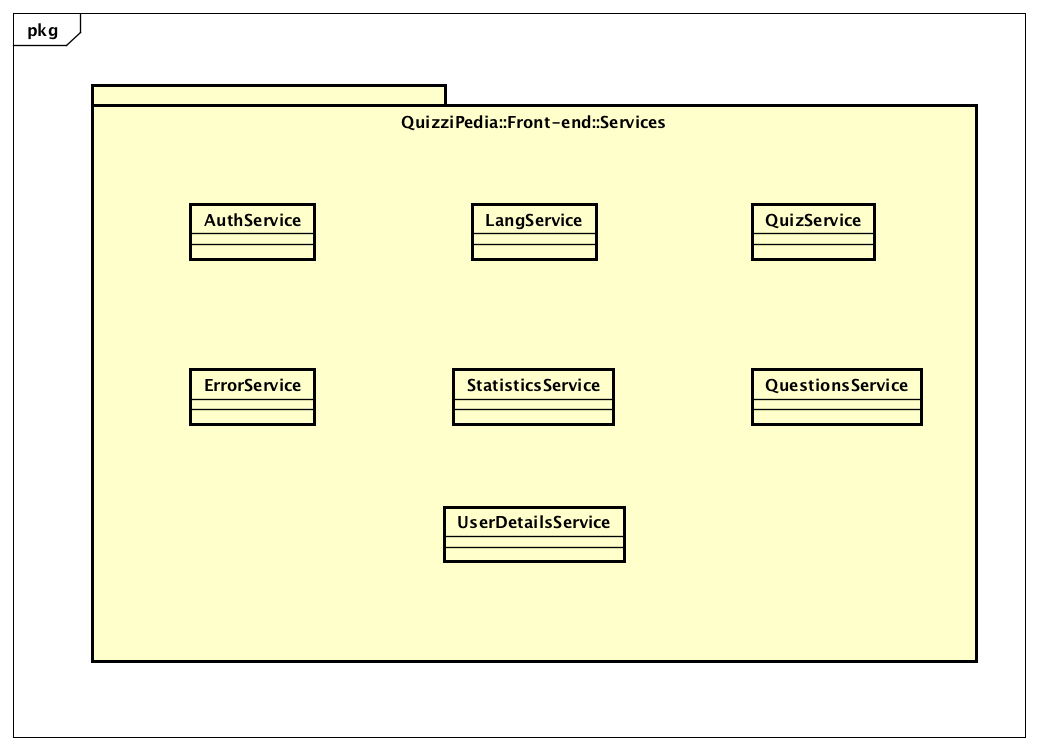
\includegraphics[scale=0.45]{UML/Package/QuizziPedia_Front-End_Services.png}
	\caption{QuizziPedia::Back-End::Services}
\end{figure}
\subsubsection{Informazioni generali}
\begin{itemize}
	\item \textbf{Descrizione} \\ Package che contiene le classi individuate che permettono la comunicazione del lato front-end con il lato back-end. 
	\item \textbf{Padre:} \texttt{Front-End}
	\item \textbf{Interazione con altri componenti:}
	\begin{itemize}
		\item \texttt{Models} - package che contiene le classi model individuate.
		\item \texttt{Controllers} - package che contiene le classi controller individuate.
	\end{itemize} 
\end{itemize}
\subsubsection{Classi}

\paragraph{QuizziPedia::Front-End::Services::AuthService}
\begin{figure}
	\centering
	%\includegraphics[scale=0.45]{UML/Package/QuizziPedia_Front-End_Services_AuthService.png}
	\caption{QuizziPedia::Back-End::Services::AuthService}
\end{figure}
\begin{itemize}
	\item \textbf{Descrizione} \\ 
	\item \textbf{Utilizzo} \\
	\item \textbf{Relazione con altre classi:}
	\begin{itemize}
		\item 
	\end{itemize}
	\item \textbf{Attributi:}
	\begin{itemize}
		\item 
	\end{itemize}
	\item \textbf{Metodi:}
	\begin{itemize}
		\item 
	\end{itemize}
\end{itemize}

\paragraph{QuizziPedia::Front-End::Services::LangService}
\begin{figure}
	\centering
	%\includegraphics[scale=0.45]{UML/Package/QuizziPedia_Front-End_Services_LangService.png}
	\caption{QuizziPedia::Back-End::Services::LangService}
\end{figure}
\begin{itemize}
	\item \textbf{Descrizione} \\ 
	\item \textbf{Utilizzo} \\
	\item \textbf{Relazione con altre classi:}
	\begin{itemize}
		\item 
	\end{itemize}
	\item \textbf{Attributi:}
	\begin{itemize}
		\item 
	\end{itemize}
	\item \textbf{Metodi:}
	\begin{itemize}
		\item 
	\end{itemize}
\end{itemize}

\paragraph{QuizziPedia::Front-End::Services::QuizService}
\begin{figure}
	\centering
	%\includegraphics[scale=0.45]{UML/Package/QuizziPedia_Front-End_Services_QuizService.png}
	\caption{QuizziPedia::Back-End::Services::QuizService}
\end{figure}
\begin{itemize}
	\item \textbf{Descrizione} \\ 
	\item \textbf{Utilizzo} \\
	\item \textbf{Relazione con altre classi:}
	\begin{itemize}
		\item 
	\end{itemize}
	\item \textbf{Attributi:}
	\begin{itemize}
		\item 
	\end{itemize}
	\item \textbf{Metodi:}
	\begin{itemize}
		\item 
	\end{itemize}
\end{itemize}

\paragraph{QuizziPedia::Front-End::Services::ErrorService}
\begin{figure}
	\centering
	%includegraphics[scale=0.45]{UML/Package/QuizziPedia_Front-End_Services_ErrorService.png}
	\caption{QuizziPedia::Back-End::Services::ErrorService}
\end{figure}
\begin{itemize}
	\item \textbf{Descrizione} \\ 
	\item \textbf{Utilizzo} \\
	\item \textbf{Relazione con altre classi:}
	\begin{itemize}
		\item 
	\end{itemize}
	\item \textbf{Attributi:}
	\begin{itemize}
		\item 
	\end{itemize}
	\item \textbf{Metodi:}
	\begin{itemize}
		\item 
	\end{itemize}
\end{itemize}

\paragraph{QuizziPedia::Front-End::Services::StatisticsService}
\begin{figure}
	\centering
	%\includegraphics[scale=0.45]{UML/Package/QuizziPedia_Front-End_Services_StatisticsService.png}
	\caption{QuizziPedia::Back-End::Services::StatisticsService}
\end{figure}
\begin{itemize}
	\item \textbf{Descrizione} \\ 
	\item \textbf{Utilizzo} \\
	\item \textbf{Relazione con altre classi:}
	\begin{itemize}
		\item 
	\end{itemize}
	\item \textbf{Attributi:}
	\begin{itemize}
		\item 
	\end{itemize}
	\item \textbf{Metodi:}
	\begin{itemize}
		\item 
	\end{itemize}
\end{itemize}

\paragraph{QuizziPedia::Front-End::Services::QuestionServices}
\begin{figure}
	\centering
	%\includegraphics[scale=0.45]{UML/Package/QuizziPedia_Front-End_Services_QuestionService.png}
	\caption{QuizziPedia::Back-End::Services::QuestionService}
\end{figure}
\begin{itemize}
	\item \textbf{Descrizione} \\ 
	\item \textbf{Utilizzo} \\
	\item \textbf{Relazione con altre classi:}
	\begin{itemize}
		\item 
	\end{itemize}
	\item \textbf{Attributi:}
	\begin{itemize}
		\item 
	\end{itemize}
	\item \textbf{Metodi:}
	\begin{itemize}
		\item 
	\end{itemize}
\end{itemize}

\paragraph{QuizziPedia::Front-End::Services::UserDetailsService}
\begin{figure}
	\centering
	%\includegraphics[scale=0.45]{UML/Package/QuizziPedia_Front-End_Services_UserDetailsService.png}
	\caption{QuizziPedia::Back-End::Services::UserDetailsService}
\end{figure}
\begin{itemize}
	\item \textbf{Descrizione} \\ 
	\item \textbf{Utilizzo} \\
	\item \textbf{Relazione con altre classi:}
	\begin{itemize}
		\item 
	\end{itemize}
	\item \textbf{Attributi:}
	\begin{itemize}
		\item 
	\end{itemize}
	\item \textbf{Metodi:}
	\begin{itemize}
		\item 
	\end{itemize}
\end{itemize}
